% all-in-one cheatsheet layout (Michael Franzen, 2013)
\documentclass[a4paper]{article}

% geometry settings
\usepackage[top=2cm, bottom=2.5cm, left=2cm, right=2cm]{geometry}

% font settings
%\usepackage[light,math]{kurier}
\usepackage[T1]{fontenc}
\usepackage[utf8]{inputenc}
\usepackage{marvosym}
\usepackage{amssymb}
\usepackage{amsfonts}
\usepackage{amsmath}
\usepackage{amsthm}

% colors
\usepackage{xcolor}
\definecolor{lightgray}{gray}{0.8}

% formatting
\usepackage{paralist}
\usepackage{multicol}
\usepackage{tabularx}
\usepackage{Tabbing}
\usepackage{booktabs}
\usepackage{fancyhdr}
\usepackage{url}
\usepackage[framemethod=tikz]{mdframed}
\pagestyle{fancy}

% math
\usepackage{array}
\usepackage{eqnarray}
\usepackage{mathtools}
\usepackage{cases}

% figures
\usepackage{wrapfig}
\usepackage{subfigure}

% figure modules
\usepackage{graphicx}
\usepackage{tikz}
\usetikzlibrary{positioning,calc, shapes}
\usepackage{algorithm2e}
\usepackage{verbatim}	

% TOC & Glossary
\usepackage{sectsty}
\usepackage[nottoc,notlof,notlot]{tocbibind}
\usepackage[titles,subfigure]{tocloft}

% commands
\usepackage{xargs}
\usepackage{ifthen}

% head line
\fancyhf{}
\chead{Graph Theory - Sheet 5 - \today\\J. Batzill (1698622), M. Franzen (1696933), J. Labeit (1656460)}
\renewcommand{\headrulewidth}{0.4pt} %obere Trennlinie

\newcommand{\sheetnumber}{1}

% (problem number)
\surroundwithmdframed[
    hidealllines=true,
    backgroundcolor=gray!10,
    skipbelow=\baselineskip,
    skipabove=\baselineskip
]{mylemma}

\surroundwithmdframed[
	linecolor=white,
	skipbelow=\baselineskip,
	skipabove=\baselineskip
]{mytheorem}

\tikzstyle{nod}= [circle, draw,inner sep=0pt, minimum size=0.5cm] 

\begin{document}
	
	\newtheorem{mytheorem}{Theorem}[section]
	\newtheorem{mylemma}{Lemma}[mytheorem]	

	\newenvironmentx*{solution}[1]{\section*{Problem #1}\addtocounter{section}{1}\setcounter{mylemma}{0}\setcounter{mytheorem}{0}}{}
	\newenvironmentx*{theorem}[1]{\begin{mytheorem}#1\begin{proof}}{\end{proof}\end{mytheorem}}
	\newenvironmentx*{lemma}[1]{\begin{mylemma}#1\begin{proof}}{\end{proof}\end{mylemma}}


	\begin{solution}{17}
		\begin{theorem}{In a planar triangulation let $n_i$ be the number of vertices of degree $i$. Then, \begin{equation*}\sum_{i \in \mathbb{N}} (6 - i)n_i = 12 \end{equation*}.}
			\begin{lemma}{Let $G = (V, E)$ and $G' = (V \cup \{v\}, E \cup E')$ be planar triangulations. Then $|E'| = 3$ and all edges in $E'$ are incident to $v$.}
			Since any planar triangulation on $n$ vertices and $e_n$ edges satisifes $e_n = 3n - 6$, we see inductively that
			\begin{align*}
				e_n &= e_{n-1} + 3& (n > 3)\\
				e_3 &= 3
			\end{align*}
			
			Since $G'$ contains $|V| + 1$ vertices, the number of edges in $G'$ exceeds the number of edges in $G$ by  $|E'| = 3$.\\
			\ \\
			Next, we will show that the degree of $v$ exceeds or is equal to $3$ and thus, all edges of $E'$ have to be incident to $v$.

			By \textsc{Kuratowski}, $G'$ is not a topological minor of $K_{3,3}$ or $K_5$ and any planar triangulation is edge-maximal. By \emph{Lemma 4.4.5 (any edge-maximal graph without topological minors $K_{3,3}, K_5$ is $3$-connected)}, $G'$ is $3$-connected.

			If the degree of $v$ deceeded $3$, then $G'$ would not be $3$-connected ($v$ could be isolated by removing two vertices) .
			
			Hence, all three edges of $E'$ are incident to $v$.
			\end{lemma}
			
			We will show by induction on the number of vertices $n$ of a planar triangulation $G$ with $n_i$ vertices of degree $i$ ($i \in \mathbb{N}$) that 
			\begin{equation*}
				T_G := \sum_{i \in \mathbb{N}} (6 - i)n_i = 12
			\end{equation*}
	.
	
			\begin{itemize}
				\item Base $\mathbf{n = 3}$
					
					Then, the graph is a triangle and the condition is satisifed:
					\begin{align*}
						T_{K_3} = \sum_{i \in \mathbb{N}} (6 - i)n_i = (6-2) \cdot 3 = 4 \cdot 3 = 12
					\end{align*}
				\item Step $\mathbf{n \geq 4}$
					
					Any $n$-vertex planar triangulation $G = (V, E)$ has a subgraph $H = (V', E')$ which is an  ($n - 1$)-vertex planar triangulation.
	
					By \emph{Lemma 1.1.1}, there is a vertex $v \in V \setminus V'$ of degree $3$. Furthermore, the degree of exactly three other vertices $v_i, v_j, v_k \in V$ is increased. Thus, $E \setminus E' = \{\{v, v_i\}, \{v, v_j\}, \{v, v_k\}\}$ and for $T_G$:
					\begin{align*}
						T_G=&T_H\\
						 &+ (6 - 3)\\
						 &+ (6 - (d(v_i) + 1)) - (6 - d(v_i)))\\
						 &+ (6 - (d(v_j) + 1)) - (6 - d(v_j))\\
						 &+ (6 - (d(v_k) + 1)) - (6 - d(v_k))\\
						=&T_H +  3 - 1 - 1 -1\\
						=&T_H\\
						=&12&\text{(by induction)}
					\end{align*}
			\end{itemize}
		\end{theorem}
	\end{solution}
	\newpage
	\begin{solution}{19}
		\begin{theorem} {A plane embedded graph on $n$ vertices that has no triangular face has at most $2n-4$ edges.}
			\begin{lemma} {Each plane triangulation ($order \geq 4$) can be modified to a plane graph containing only faces of order $4$ by removing one edge for each two faces}
				
				Proof by induction over the order of a plane triangulation $G$:\\
				\begin{itemize}
					\item \textbf{Base: $V(G)=4$}\\
						G contains of $4$ faces $f_1,f_2,f_3,f_4$. We get the desired graph by removing the shared edge between $f_1, f_2$ and $f_3, f_4$.
						This is possible because each face is adjacent to one another. The remaining graph is, as desired, created by removing one edge foreach $2$ faces.
						
					\item \textbf{Step: $V(G)=n$}\\
						Let $G' = G -\{u\} ~ (u \in V(G)$ with $deg(u) = 3$ as shown in $\textbf{Lemma 1.1.1})$. Then $G'$ is still a plane triangulation and the amount of faces in $G$ is exactly $2$ more than in $G'$, because by removing the vertex $u$, $3$ edges were removed, thus, $2$ triangular faces were removed.\\
						By induction we get the desired graph $H'$ for $G'$ by removing one edge for each $2$ faces. Moreover, by inserting $u$ and its $3$ adjacent edges in $H'$ at their old position, $2$ faces of degree $3$ were created (Would there be more than $2$ new faces, the face in which $u$ was inserted would have an order of at least $5$). Thus, there are only two faces of order $3$ remaining. Because all inserted edges are incident to $u$, these two faces of oder $3$ are adjacent and can be merged by removing the shared edge.\\
						The resulting graph of order $n$ is still plane (only edges have been removed), has only faces of order $4$ and was created of $G$ by removing one edge for each $2$ faces. 
					
				\end{itemize}
			
			\end{lemma}
		
			\begin{lemma} {Each plane graph with no triangular face can be modified to a plane graph containing only faces of order $4$  and with at least the same amount of edges}
				Let $G$ be such a plane graph with no triangular face. Let $G'$ be the plane triangulation of $G$.\\
				To get $G'$ out of $G$ edges have to be added. Because the smallest face is of order $4$, at least $1$ edge for each face is needed to reduce the size of all faces, resulting in at least one additional face for each existing face in $G$, to be more precisely, in exactly one additional face for each inserted edge. So $G'$ has at least twice as much faces as $G$ and exactly one new edge for each new face. As shown in \textbf{Lemma 2.1.1}, $G'$ can be modified to a plane graph $H$ containing only faces of order $4$ by removing one edge for each two faces. Thus, the amount of faces in $H$ is at least as much as in $G$, and furthermore the amount of edges is at least as much as in $G$, because for each two faces exactly one edge has been removed.\\
				All in all, $H$ is a graph containing only faces of order $4$ and has at least the same amount of edges as $G$.
			\end{lemma}		
			
	
			Let $G=(V,E_G)$ be a plane graph with no plane triangulation.\\
			As shown in \textbf{Lemma 2.1.2}, we get a plane graph $H=(V,E_H)$ ($F_H$ corresponding faces, each face of order 4), containing at least the same amount of edges as $G$ and the same set of vertices $V$.\\
			
			By $Euler's Formula$ and the fact $|E_H|= \frac{4 * |F_H|}{2}$ (because each face in $F_H$ has order 4 and each edge is exactly counted twice), we get the following:\\
			$2 = |V| - |E_H| +|F_H|$ $\leftrightarrow$ $2 = |V| - |E_H| + \frac{E_H}{2}$ $\leftrightarrow$ $|E_H| = 2 * |V| - 4$.\\
			This inequality allows us to bound the amount of edges as following:\\\\
			$|E_G| \leq |E_H| = 2 * n - 4$   $~~(n=|V|)$
			
		\end{theorem}
	\end{solution}
	\newpage
	\begin{solution}{20}
		\begin{theorem}{For a planar embedded graph $G$ on $n$ vertices such that $G* \cong G$, the number of edges $e = 2(n - 1)$.}
			The faces of $G$ corrospond to the vertices of $G^*$. Considering their ismorphism, the number of faces $f$ of $G$ equals the number of vertices of $G$.
			
			$G$ is planar, by \emph{Euler's Characteristic}: $n - e + f = 2 \Rightarrow 2n - e = 2 \Rightarrow e = 2(n-1)$. \\
			How to find such a graph $G=(V,E)$ which is isomorph to it's plane dual $G*$ with $|V| = n \geq 4$. 
			Let $v_2,v_3,...v_n$ be a simple cycle with $v_1$ connected with an edge to every other vertex. 
			$G$ can be planar embedded by drawing $v_1$ in the middle of the cycle. 
			We can see that $G \cong G*$ holds by finding a bijection identifying every vertex of $G$ with exactly one face of $G$. 
			The vertices $v_2,v_3...v_n$ can be identified with the face below it. 
			The vertex $v_1$ can be identified with the face surrounding $G$. 
			Now it is easy to see that $G \cong G*$ holds. 
			\begin{center}
			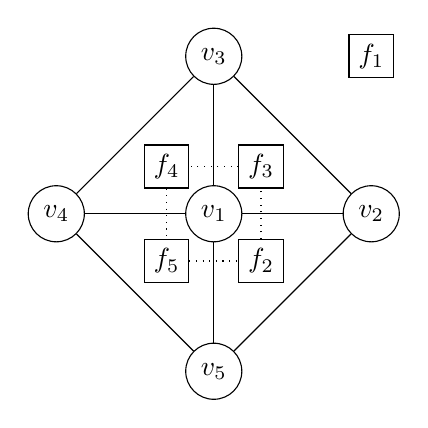
\begin{tikzpicture}
				\node[circle, draw] (v1) at (0, 0) {$v_1$};
				\node[circle, draw] (v2) at (2, 0) {$v_2$};
				\node[circle, draw] (v3) at (0, 2) {$v_3$};
				\node[circle, draw] (v4) at (-2, 0) {$v_4$};
				\node[circle, draw] (v5) at (0, -2) {$v_5$};
				\node[draw] (f1) at (2.0, 2.0) {$f_1$};
				\node[draw] (f2) at (0.6, -0.6) {$f_2$};
				\node[draw] (f3) at (0.6, 0.6) {$f_3$};
				\node[draw] (f4) at (-0.6, 0.6) {$f_4$};
				\node[draw] (f5) at (-0.6, -0.6) {$f_5$};

				\draw(v1) -- (v2);
				\draw(v1) -- (v3);
				\draw(v1) -- (v4);
				\draw(v1) -- (v5);
				\draw(v2) -- (v3);
				\draw(v3) -- (v4);
				\draw(v4) -- (v5);
				\draw(v5) -- (v2);
				
				\draw[dotted](f2) -- (f3);
				\draw[dotted](f3) -- (f4);
				\draw[dotted](f4) -- (f5);
				\draw[dotted](f5) -- (f2);
			\end{tikzpicture}
			\end{center}
			
		\end{theorem}
	\end{solution}
	
\end{document}
